\documentclass[letterpaper, 12pt]{math}

\usepackage{tikz}

\title{CSCI 251: Concepts of Parallel and Distributed Systems}
\author{Alvin Lin}
\date{October 23rd, 2017}

\begin{document}

\maketitle

\section*{Time and Global State}
Topics:
\begin{itemize}
  \item Clocks - Physical, Logical, Vector
  \item Events
  \item Processes
  \item Consistent Cuts
  \item Global States
\end{itemize}

\subsection*{Clocks}
\textbf{Skew:} the difference between two clocks. \\
\textbf{Drift:} the change in the frequency of the oscillation of a clock. \\
\textbf{UTC:} Coordinated Universal Time \\
Logical clocks: for any process \( p_i: e \to_{i}e' \) implies event \( e \)
happens before \( e' \) on process \( i \). For any message \( m_1: send(m)\to
receive(m) \). When a process \( p_i \) sends a message `m' to another process,
it piggybacks on `m' the value \( t = L_i \). If \( e\to e' \) and \( e'\to e''
\), then \( e\to e'' \).
\begin{center}
  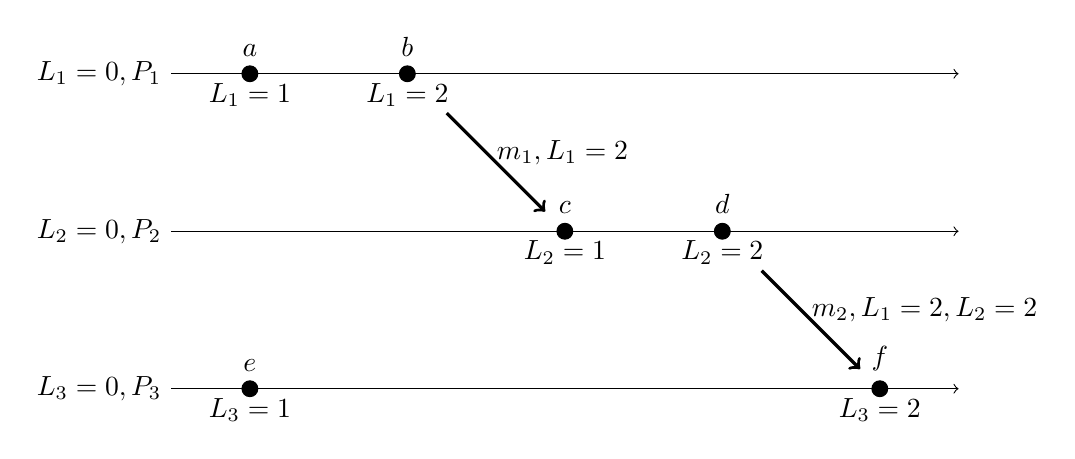
\begin{tikzpicture}
    \draw[<-] (10,0) -- (0,0) node[left] {\( L_1 = 0, P_1 \)};
    \draw[<-] (10,-2) -- (0,-2) node[left] {\( L_2 = 0, P_2 \)};
    \draw[<-] (10,-4) -- (0,-4) node[left] {\( L_3 = 0, P_3 \)};
    \draw[fill=black] (1,0) circle (0.1cm) node[above, yshift=0.1cm] {\( a \)}
      node[below] {\( L_1 = 1 \)};
    \draw[fill=black] (3,0) circle (0.1cm) node[above, yshift=0.1cm] {\( b \)}
      node[below] {\( L_1 = 2 \)};
    \draw[->,very thick] (3.5,-0.5) -- (4.75,-1.75)
      node[pos=0.4,right] {\( m_1, L_1 = 2\)};
    \draw[fill=black] (5,-2) circle (0.1cm) node[above, yshift=0.1cm] {\( c \)}
      node[below] {\( L_2 = 1 \)};
    \draw[fill=black] (7,-2) circle (0.1cm) node[above, yshift=0.1cm] {\( d \)}
      node[below] {\( L_2 = 2 \)};
    \draw[->,very thick] (7.5,-2.5) -- (8.75,-3.75)
      node[pos=0.4,right] {\( m_2, L_1 = 2, L_2 = 2 \)};
    \draw[fill=black] (1,-4) circle (0.1cm) node[above, yshift=0.1cm] {\( e \)}
      node[below] {\( L_3 = 1 \)};
    \draw[fill=black] (9,-4) circle (0.1cm) node[above, yshift=0.1cm] {\( f \)}
      node[below] {\( L_3 = 2 \)};
  \end{tikzpicture}
\end{center}

\subsubsection*{Vector Clocks}
\[ V = [V_1,V_2,V_3] \]
\( V_i = [j] \) represents the vector clock on process \( i \) with the entry
for process \( j \). Each clock maintains what it knows of the state of other
clocks.
\begin{center}
  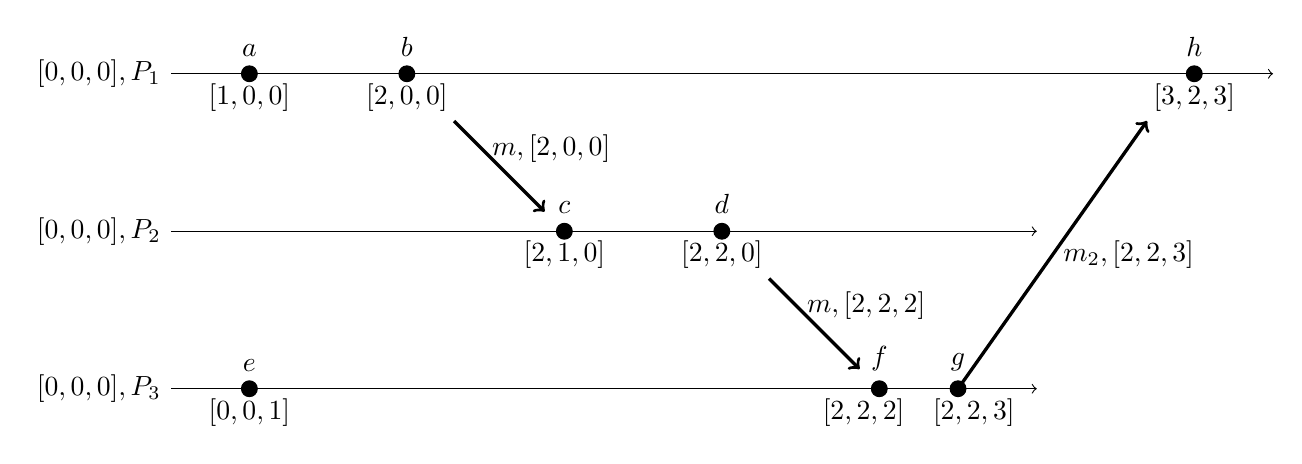
\begin{tikzpicture}
    \draw[<-] (14,0) -- (0,0) node[left] {\( [0,0,0], P_1 \)};
    \draw[<-] (11,-2) -- (0,-2) node[left] {\( [0,0,0], P_2 \)};
    \draw[<-] (11,-4) -- (0,-4) node[left] {\( [0,0,0], P_3 \)};
    \draw[fill=black] (1,0) circle (0.1cm) node[above, yshift=0.1cm] {\( a \)}
      node[below] {\( [1,0,0] \)};
    \draw[fill=black] (3,0) circle (0.1cm) node[above, yshift=0.1cm] {\( b \)}
      node[below] {\( [2,0,0] \)};
    \draw[->,very thick] (3.6,-0.6) -- (4.75,-1.75)
      node[pos=0.3,right] {\( m,[2,0,0] \)};
    \draw[fill=black] (5,-2) circle (0.1cm) node[above, yshift=0.1cm] {\( c \)}
      node[below] {\( [2,1,0] \)};
    \draw[fill=black] (7,-2) circle (0.1cm) node[above, yshift=0.1cm] {\( d \)}
      node[below] {\( [2,2,0] \)};
    \draw[->,very thick] (7.6,-2.6) -- (8.75,-3.75)
      node[pos=0.3,right] {\( m,[2,2,2] \)};
    \draw[fill=black] (1,-4) circle (0.1cm) node[above, yshift=0.1cm] {\( e \)}
      node[below] {\( [0,0,1] \)};
    \draw[fill=black] (9,-4) circle (0.1cm) node[above, yshift=0.1cm] {\( f \)}
      node[below, xshift=-0.2cm] {\( [2,2,2] \)};
    \draw[fill=black] (10,-4) circle (0.1cm) node[above, yshift=0.1cm] {\( g \)}
      node[below, xshift=0.2cm] {\( [2,2,3] \)};
    \draw[->,very thick] (10,-4) -- (12.4,-0.6)
      node[pos=0.5,right] {\( m_2,[2,2,3] \)};
    \draw[fill=black] (13,0) circle (0.1cm) node[above, yshift=0.1cm] {\( h \)}
      node[below] {\( [3,2,3] \)};
  \end{tikzpicture}
\end{center}
Initially, \( V_i[j] = 0 \) for \( i,j = 1,2,\dots N \). Just before \( P_i \)
timestamps an event it increments \( V_i[i] \). \( P_i \) includes the value
\( t = V_i \) in every message it sends. When \( P_i \) receives a timestamp
\( t \) in a message it sets \( V_i[j] = max(V_i[j],t[j]) \) for
\( j = 1,2,\dots N \).

\section*{Reminders}
\noindent Professor Mohan Kumar: \\
\url{mjkvcs@rit.edu} \\
\url{https://cs.rit.edu/~mjk} \\

\noindent Rahul Dashora (TA): \\
\url{rd5476@mail.rit.edu} \\

\begin{center}
  You can find all my notes at \url{http://omgimanerd.tech/notes}. If you have
  any questions, comments, or concerns, please contact me at
  alvin@omgimanerd.tech
\end{center}

\end{document}
